\chapter{可挂载完整性保护树:Mountable Merkle Tree}

在前面几张中,我们详细介绍了已有的完整性保护方案,包括了最新颖的VAULT ~\cite{taassori2018vault}。这些工作的一个共同点是希望通过增加树中节点的扇出来减少树的深度,同时进一步
优化运行时候的检查的开销。然而盲目增加树节点的扇出会带来安全隐患(重放攻击等等),在最新颖的完整性保护方案VAULT中,树中节点的扇出24(第三层及以上),同样
无法保护TB级别的内存数据。在本文中,我们提出了一种新的完整性保护数据结构:哈希森林以及可挂载完整性保护树(Mountable Merkle Tree)。希望通过新的完整性保护数据结构,能够实现一下几点:
\begin{itemize}
    \item 支持TB级别的内存完整保护
    \item 支持动态的内存完整保护分配机制
    \item 支持离散的内存保护
    \item 可以接受的运行时开销
    \item 实现保护内存的可扩展性
\end{itemize}
可挂载完整性保护树(MMT)以及哈希森林,能够很好的解决当下安全领域一些热点问题:Enclave的内存完整性保护以及NVM中的数据保护。同时该方案也能够和已有的完整性保护结合,具有较好兼容性。

\section{哈希森林,子树与根树}
已有的完整性保护方案都采用了哈希树的方式管理哈希(hash)或者计数器(counter),树的组织结构能以较小的开销,保护大量的内存数据;但是随着需要保护的数据越来越大,哈希树只能够通过增加树的深度来保护更多的内存。
然而增加树的深度会带来更大运行时的性能开销,这也是之前工作的共同缺陷所在。我们认为,增加保护的内存大小不仅仅只能通过增加树的深度来实现,增加树的个数,同样也能够保护更多的内存,同时
也不会增加运行时的开销。在本篇论文中,我们提出了哈希森林的概念,哈希森林中由一组哈希树构成,每一棵哈希树都能够保护一块物理内存,如果需要保护更多的物理内存,只需要往哈希森林中增加更多的
哈希树即可;同样如果需要保护的内存减少,那么只需要将哈希树从哈希森林中移除。哈希森林具有以下几个特性:一、实现动态可扩展的内存完整性保护;二、通过增加哈希树的个数来增加保护内存的大小;三:支持TB级别内存完整性保护。

哈希森林的一种简单的实现,是保护更多的哈希树的根节点,然后正如我们之前所提的,验证者不希望保护大量的数据,而完整性保护中,即内存控制器(memory controller)中的空间有限,只能保存少量的哈希值或者计数器值
所以如果仅是简单保护更多的哈希树根节点,显然没有办法达到期望的具有可扩展性的内存保护,因为保护的内存大小受到内存控制器中能够保存的根节点数量的限制。为了实现可扩展的内存保护,我们提出了两个新的概念:\textbf{子树}和\textbf{根数}。
我们认为整个哈希森林由子树和根树组成。子树即哈希森林中所有的可以动态加入或者移除的哈希树,一棵棵子树构成了哈希森林;根数则保护哈希森林的完整性。所以我们只需要把根数的根节点:Root-of-root保护在内存控制器中即可,而不需要保护所有的子树根节点。
因为内存控制器中的空间有限,我们无法将所有的子树节点放在内存控制器中,相反我们把所有的子树的节点以及根节点保存在内存中,我们将所有子树的根节点放在一块特殊的内存空间:MMT元数据区域(之后会详细介绍)。内存中的空间被认为是充足的,我们可以存储足够多的子树。当然在内存控制器中仅仅只放根树的根节点是不够,这样会退化成为之前的完整性保护方案,即仍然只存在一棵树。

为了将哈希森林结合到内存控制器中,我们首先对内存的访问做了调研。我们发现,CPU对内存的访问具有一定的局域性,即在一段时间内,CPU可能访问某一部分的内存数据,而不会随机的访问整个内存空间。这个观察结果已经广泛的使用在了计算机体系结构中,比如cache的提出就是为了缓解CPU频繁的访问
内存中的数据,既然内存中的数据可以通过cache来提升性能,那么我们也可以采用同样的方式缓存子树的根节点。我们首先将所有的子树的分为三类:
\begin{enumerate}
  \item 活跃的子树:即CPU正在访问该子树保护的内存数据或者刚刚访问了该子树保护的数据。
  \item 不活跃的子树:该子树对应的内存数据需要被保护,但是当前或者近段时间内,该内存数据没有被CPU访问。
  \item 未分配的子树:未分配的子树表示内存的数据不需要经过保护。
\end{enumerate}
首先活跃的与不活跃的子树的节点都需要在内存中有备份,如果该子树是活跃的,那么我们将该子树的根节点缓存在内存控制器中,CPU可以直接在内存控制器
中读到子树根节点的哈希值或者计数器值。如果CPU访问的子树不活跃,我们在后续段落中做进一步的讨论。综上,我们提出了哈希森林,子树和根数等概念,我们通过增加哈希森林中子树的个数来保护更多的内存。为了节省内存控制器中的空间,我们只需要保护根数的根节点,为了在大多数检查
中只需要检查子树的节点,我们将当前活跃的子树根节点缓存在内存控制器中,这样对内存的检查不需要从根数的根节点开始,只需要从子树开始即可,来实现增加内存大小,但在大多数情况下不增加检查时访问树的深度。下面我们将从内存完整性保护架构中的不同部分,以及MMT的管理机制等方面做具体的阐述。

\section{内存控制器}
内存控制器控制对内存的访问,内存控制器是SoC上的一个单元,CPU中的访存指令在cache中如果没有命中,或者cache中发生了cache miss等事件,需要从内存中读取或者写入数据的时候,就会向内存控制器中发送一个包的请求。内存控制器解析包请求,然后通过总线将需要读取或者写入的数据的物理地址(数据)以包的形式发给DIMM,
DIMM中的控制器相应请求,写入或者返回对应内存地址上的数据。在一个CPU上可以拥有多个内存控制器单元,每一个内存控制器通过总线控制一个DIMM,通过多个内存控制器,能够实现并发的内存操作。CPU会协调不同的内存控制器,使其能够高效协同工作。为了在访问内存的时候保证内存数据的完整性,我们需要在
内存控制器中做一定的修改。传统的完整性保护架构中,只需要在硬件中实现对完整性保护树的索引,取值,更新与哈希计算。在MMT中因为引入了哈希森林,所以还要加上对子树的管理,分配等其他功能。在MMT的内存控制器中我们增加了三个组件:1、安全比特表(Secure Bitmap);2、
子树缓存(Mount table);3、根树根节点哈希/计数器(Root-of-root),如图~\ref{fig:MMT-arch.png}所示。
\begin{figure}[!htp]
    \centering
    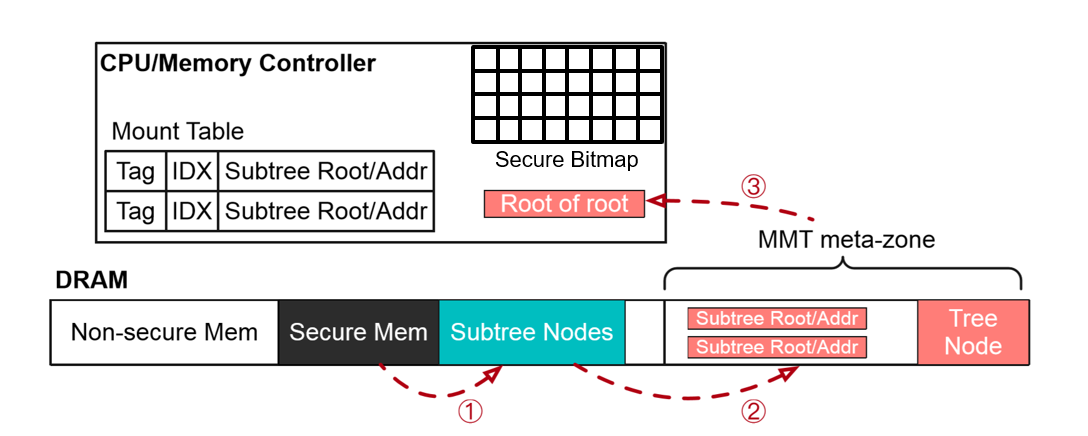
\includegraphics[scale=0.7]{MMT-arch.png}
    \caption{\textbf{MMT中内存控制器与内存布局}。\emph{Secure Bitmap}记录了当前已经分配的子树,\emph{Mount Table}记录当前活跃的子树根节点,\emph{Root-of-root}根树的根节点(可信基)。内存布局:
    \emph{Non-secure Mem}非安全内存,\emph{Secure Mem}安全内存,\emph{Subtree Node}子树节点,\emph{MMT metadata zone} MMT元数据区域}
   \label{fig:MMT-arch.png}
\end{figure}

\textbf{安全比特表:Secure Bitmap}
安全比特表用于记录哪些子树已经分配了,在之后的章节中我们会详细的介绍内存中的布局。安全比特表用一个比特来代表其对应的子树是否被分配,活跃的子树以及不活跃的子树都是已经分配的子树,而未分配的子树对应的内存无需完整性保护。安全比特表的开销取决总内存的大小以及
子树的大小,考虑到一棵能够保护4M大小的子树以及总内存为512G,,那么对应内存控制器中的安全比特表的大小只需要16K。16K的大小对于现在内存控制器来说是完全可以接受的,如果子树保护的内存更多情况下,安全比特表的开销将进一步的减少。当安全比特表中的
比特为1,说明对应的子树已经分配,需要完整性保护的检查,如果未被分配,说明是正常的内存,不需要进行完整性的保护。通过安全比特表这个概念,我们可以实现动态安全内存的分配,而不需要事先指定需要保护的内存区间。安全比特表也可以被其他的组件
所代替,比如CPU对内存的访问可以带上一个特殊的标志位,如果该标志位是1则说明访问的是需要完整性保护的内存,反之则是正常的内存。通过这样的机制我们可以实现更加细粒度的内存区分,在之后的章节中我们会详细的介绍如何按照页的粒度进行完整性保护。

\textbf{子树缓存:Mount Table}
参考内存中缓存的数据结构,我们在内存控制器中增加子树缓存。子树缓存类似与内存中cache的结构,也分成多个集合,每一个集合中又包括了多路的子树缓存行,每一个子树缓存行中存在对应的tag,index,以及4个条目的子树根节点。同时每一个子树缓存集合中
还包括了LRU等相关信息,用于子树的驱逐策略。子树的根节点主要有两部分组成的,一部分是子树哈希/计数值,另一部分是子树在内存中所处的位置。之所以需要增加一个子树在内存中所处的位置,是因为子树是可以动态的分配的,我们不能事先给子树确定
一块内存空间,所以当一条内存访问指令来的时候,我们需要通过子树的地址来确定子树在内存中的位置,从而通过子树进行完整性保护的检查。子树的根节点大小总共为16byte。首先子树根节点的大小必须能够整除一条缓存行的大小。在这里缓存行的大小为64B,同属
内存控制器也是按照64B的大小进行内存的读写操作,所以16B刚好是一条缓存行的四分之一;另外按照实际上更节点中的计数值以及哈希/计数值的大小可以压缩到8 byte,但是考虑到我们方案的通用性,以及之后的延展性,我们这里将一棵子树的根节点大小设置为16 byte。
当CPU向内存控制器发送一个请求的数据包的时候,内存控制器能够解析该请求包。首先内存控制2器会将该请求的物理地址转换为对应的内存块。正如之前所说的,缓存行的大小以及内存块的大小都是64B,所以我们对内存的读写都需要以64B对齐。将CPU发出的内存
指令以64B对齐之后,内存控制器会索引内存块落在按一个子树中,内存控制器能够得到对应的子树编号(假设我们子树的大小是4M,那么0-4M的内存块都由编号为0的子树保护)。子树的编号可以进一步拆分为:tag+index+offset。tag是用于区分在同一个缓存集合中的不同的
缓存行,index表示该子树是属于哪一个缓存集合的,offset用于表示当前的子树属于一个缓存行中的第几个子树(因为一个缓存行中有4个子树的根节点)。以上的方式和计算机中cache的组织结构非常相识,同时我们对子树缓存的驱逐策略采用了LRU的方式,即我们淘汰
最老的为被访问到的缓存行。LRU的策略能够通过增加一个比特位实现,内存控制器一旦访问了某个缓存行,就将对应的缓存行的LRU比特置为1,当子树缓存行不够的时候,LRU从上一次淘汰的缓存行开始,如果LRU比特是1那么就将它清零,如果LRU比特是0那么就驱逐该缓存行
并且记录该位置。在子树缓存中保存了当前活跃的子树,缓存的大小决定了内存控制器中能够保存的活跃子树的大小,在该系统中,内存控制器中保存了32棵子树,能够支持128M的内存保护,这个大小和SGX中保护的内存的大小一致。在云场景中,内存控制器中保护的子树根节点
个数可以更多,一支持更多的活跃子树,减小运行时候的开销。

\textbf{Roor-of-root}
Root-of-root是根数的根节点的哈希/计数值,不同于子树缓存:Mount Table,Root-of-root中的数值常驻在内存控制器中,但是与Mount table不同的是,Root-of-root可以非常小,往往只有几个bit。Mount  table中空间不够的话的子树根节点会采用LRU的淘汰策略,将
子树根节点淘汰到内存中。Root-of-root只存在一个,并且在内存中并不存在备份。所以该值被固定在内存控制器中,以防止被恶意的攻击者篡改,Root-of-root是整个完整性检查系统的可信基础。

内存控制器中新增加三个部件:Secure Bitmap;Mount Table;Root-of-root,同时在内存控制器中还需增加完整性保护的逻辑以及挂载子树的功能,这些将在之后的章节中详细的介绍。

\begin{figure}[!htp]
  %  \setlength{\abovecaptionskip}{-5pt}
    \centering
    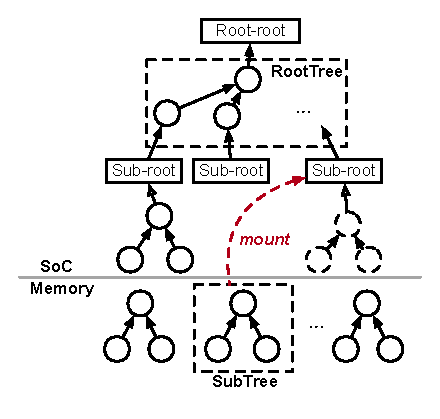
\includegraphics[scale=1]{fig/design-hw-mountable-tree.eps}
    \caption{\textbf{哈希森林}}
    \label{fig:hash-forest}
    %, and the common root ancestor (the topmost node) is fixed in the SoC.
  \end{figure}
\section{完整性保护树的动态原语}
之前所有的工作中,完整性保护树都是静态的,不同于其他的树的组织结构,因为可以动态的增加一个分支,或者合并两个分支。完整性保护树不能够更改树的组织结构,因为内存控制器需要在获得内存地址的时候就知道其对应的每一层节点的在内存中具体位置,静态的树的组织结构能够不改变
树中的每一层的结构以及对应所在的位置中,所以树中节点的位置在初始化的时候就能够确定了,方便内存控制器之后的读取与验证。静态的树在实现的时候虽然很简单,但是存在诸多弊端,比如只能够保护连续的内存空间,没有办法动态的更新保护的内存范围。所以我们希望给静态的完整性保护树
附上一些动态操作的原语,能够实现动态的内存你保护,同时让内存控制器能够快速的知道树中每个节点在内存中的位置。结合在上诉的活跃子树与不活跃子树的描述与分析,我们为Mountable merkle tree和哈希森林提出四个动态操作原语:挂载(Mount),卸载(Unmount),添加(add)和移除(remove)。
通过这四个原语,我们可以加子树在活跃,不活跃与未分配三种状态间转换。如图~\ref{fig:hash-forest}所示,挂载(Mount)与卸载(Unmount)分别对应将子树的状态从活跃转换为不活跃以及从不活跃转换为活跃。挂载与卸载的想法类似与在操作系统中的文件系统中的挂载文件到文件树中。在Mountable merkle tree中,我们可以将
一棵子树挂载到Mount Table中,在Mount Table中的子树的根节点以及子树的地址,能够被内存控制器直接读到,从而进行完整性保护的计算。而卸载的操作可以将一个挂载在Mount Table中的子树卸载到内存中,这样可以奖Mount Table中的空间留给其他的活跃的子树使用。
添加与移除是针对分配与未分配子树而言的。添加操作是将子树添加在哈希森林中,同时奖secure bitmap中对应的子树的比特为设置成为1,一棵子树添加到哈希森林中并不意味着他是活跃,而是处于不活跃的状态。同样我们也可以使用移除(remove)操作将一棵子树从哈希森林中移除,这个操作
意味的该子树对应的内存不需要经过完整性保护。通过这四个完整性保护树的动态操作原语。我们可以实现动态的增加需要保护的内存,把活跃的子树挂载到Mount  Table中来减少运行时候的开销。同时在添加一棵子树到哈希森林中的时候,我们需要指定该子树在内存中的位置,并且和子树初始化的哈希/计数值
保存在内存中的一块特殊的区域:MMT元数据区域中,之后在挂载的时候,会将该子树的地址写入Mount Table中,这样内存控制器就可以知道该子树的其他节点在内存中的位置,不依赖与任何运行时的信息。

\section{内存布局}
如图~\ref{fig:MMT-arch.png}所示,为了适应动态可扩展的内存完整性保护,我们对内存中的布局做了进一步的细分。内存中的居于被分为四个部分,分别是:非安全内存,安全内存,子树节点区域以及MMT元数据区域。其中非安全内存不需要经过完整性验证,其对应的子树属于未分配的状态;安全内存是指该内存受完整性保护,它对应的子树处于已分配
状态,但是不能保证子树一定处在活跃的状态;子树节点区域中存放着子树的中间节点,子树的根节点存在内存控制器中,但是因为内存中的空间是有限,不可能存下子树中的所有的节点,所以子树中的中间节点需要存放在内存中。子树节点区域可以动态的分配,往往实在动态添加安全内存的时候随之一起指定对应的子树
节点区域。安全内存以及子树节点区域可以离散的分布在内存中,不一定需要时连续的内存区间。MMT元素据区域(MMT metadata zone)是一块特殊的区域,该区域只能由拥有特权级的程序访问以及修改,MMR元素剧区域中存储着所有的子树的根节点(包括了未分配即已分配的子树),根节点中包括了对应子树的哈希/计数值
以及子树的在内存中地址,如果当前的子树没有分配,那么子树的根节点中的哈希以及地址为空。MMT元素据区域中的另一部分时根数的节点。根数用来保护MMT元素据区域中所有子树的根节点的完整性。如果恶意的攻击者通过物理攻击方式修改MMT元素据区域中的数据将会被根数的检查发现,如果攻击者通过软件攻击的方式
修改MMT元素据区域中的值将会被禁止,只有特权程序才能访问该区域,其他程序想要修改将会被禁止。下面我们将具体的介绍一下在RISCV架构中如何保护MMT元素据区域的

\textbf{监视者(Monitor): }在RISCV的指令集架构中分为四个特权级,分别时用户态(U mode),内核态(S mode),虚拟化层(H mode),监视器层(M mode)。其中U mode中运行着一般的用户程序,S mode中运行着操作系统,H mode中运行着虚拟机管理者(VMM),M mode中运行的监视器。其中M mode拥有最高的特权级。M mode可以访问所有的物理资源
以及拥有自己的特权指令。M mode中的代码非常少,一般情况下会把对物理资源的管理交给更低权限的程序例如运行在S mode中内核程序,或者运行在H mode中的VMM。正常的M mode中值运行了启动机器的bootloader用于加载代码,以及少量的初实话工作。当然我们可以在M mode中加入一个监视着(monitor)来监管部分物理资源或者
对其作检查,来提高系统的安全性。在RISCV的指令集架构中,存在着一些特殊的寄存器:pmp。pmp寄存器时成对出现的,包括一个pmp地址寄存器以及一个pmp配置寄存,通过这两个寄存器,可以划初内存中的一块连续的内存区域,同时给该内存区域设置上访问的权限,在RISCV指令集中pmp寄存一般由16个,既可以划分出16个连续独立的内存区域。我们利用M mode中的监视器以及pmp寄存器来保护MMT 元素据区域。
首先我们选定一个pmp寄存器,然后给它分配一块物理内存作为MMT元素据区域。并且给该内存设置的访问修改的权限为M mode,即只有处在M mode中的程序才能够访问MMT 元素据区域中的信息。其他的特权级的程序如果访问该内存区域将会下陷到M mode中进行处理。通过这样的机制能够保证只有M mode中改的监视者能够修改MMT 元素据区域中的数据
其他任何的程序都无法修改其中的数据。从而保证了MMT 元数据区域不会受到软件攻击。

\section{完整性检查流程}
下面将详细介绍如何进行完整性检查:
\begin{enumerate}
    \item CPU向内存控制器发送一个内存访问请求的包,内存控制器解析该内存访问的地址属于哪一个子树,然后再secure bitmap中检查该子树是否被分配,该内存访问是否落在安全内存中。如果落在安全内存中着进入步骤二,否者直接进入步骤六。
    \item 内存控制器检查访问地址对应的子树是否再Mount Table中(通过检索index以及匹配tag),如果子树再Mount Table者进入步骤五,否者进入步骤三
    \item 子树不在Mount Table中,所以内存控制器根据LRU的方式选择一个合适的子树缓存行,将其中的子树的根节点淘汰到内存中MMT 元素据区域中(一个子树缓存行中存储了四个连续的子树的根节点)。因为被淘汰到内存中的子树根节点中的数据可能发生变化,所以会更新根书中节点的数值,如果必要的话会更新内存控制器中的Root-of-root中的数值常驻在内存控制器中,但是与Mount。
    \item 内存控制器选择目标地址对应的子树,将子树挂载到Mount table中。再读取相应的子树的时候,需要将依据根数中节点哈希/计数值对MMT 元数据区域中的子树根节点数据进行完整性验证,如果验证通过才能够将子树根节点加载到Mount Table中,因为一旦加载之后,对子树的访问将不会触发对根数的检查。
    \item 现在对应子树的根节点已经在Mount Table中了,我们根据子树根节点中的哈希/计数值和子树的物理地址,找到对应的子树节点区域,然后通过子树根节点中改的哈希值,对访问内存中的数据进行完整性检查。如果检查通过则进入步骤六
    \item 内存控制器对访问的内存进行读取操作,如果是读操作,那么将该内存块中的数据以及读出来然后用包的形式返回给CPU,如果是写操作,那么将对应的数据写道内存块中,更新内存中的数值。
\end{enumerate}
以上的步骤是MMT中为了自动实现挂载以及卸载操作所增加的内存完整性检查流程。下面会具体阐述如果通过Mountable merkle tree进行完整性检查,这个部分在上述步骤中的三四五中使用到,首先我们会具体介绍Mountable merkle tree中节点的组织结构。

\subsection{树节点结构:三级counter}
下面我们会详细的介绍Mountable merkle tree中节点的组织形式。一个节点的大小为512比特,符合一条缓存行的大小,这一点是为了方便能够把整个节点缓存在系统的cache中减少读内存的操作。一个树节点的512bit被分成了五个部分,分别是:global counter,extra counter,index,local counter以及hash。首先将介绍global conuter以及local counter的作用。
首先,为了提高节点中的扇出,我们用counter替代了hash,这个做法在BMT中得到的使用,用counter代替hash能够很好兼顾加密以及完整性的保护,我为了减少受到replay攻击的可能,每一次对内存的写访问都会增加对应的counter的值。采用global counter和local counter的方式是在VAULT中首次提出在完整性保护中的。local counter决定了一棵树节点的扇出的度数,而global counter决定了counter的大小(counter的大小是防止重放攻击的关键)。
每一个树节点的counter是由local counter和global counter拼接而成,所有的local counter公用一个glocal counter,一旦local counter耗尽了,需要增加global counter数值时,就会使所有节点中的counter的数值均发生了变化,进而所有被counter保护的子节点都需要重新计算对应的哈希。重新计算哈希将带来不可忽略的开销,所以我们尝试优化树节点中的数据结构来缓减这部分的性能开销。

\begin{figure}[!htp]
  \centering
  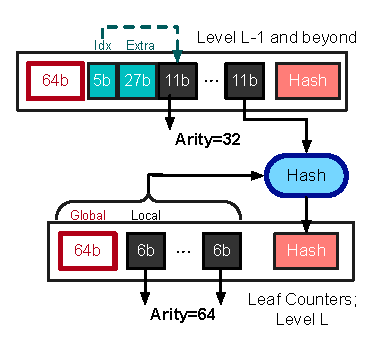
\includegraphics[scale=1]{fig/design-hw-mountable-tree-layout.eps}
  \caption{\textbf{MMT树节点数据结构:}三级counter}
 \label{fig:three-level-count.png}
\end{figure}

同Mountable merkle tree的想法类似,我们发现,在完整性保护树中,也存在一定的局域性,树中的节点被分成了热节点以及冷节点,其中热节点是快速增长的counter节点,冷节点是慢速增长的counter节点,因为树的组织形式,一个父节点将会对应多个子节点,即父节点保护的内存范围比子节点要大,在树的顶部的节点中,往往只会存在一个活跃的节点,又因为树中顶部的节点被访问的概率远超过
底部的节点,所以counter会快速的增长,更加容易发生overflow,所以我们区分对待同一个树节点中的不同的counter。在一个树节点中可能存在一个或者少数几个快速增长的counter节点,剩下的counter的节点是不活跃的节点,增长的速率比较慢,根据以上的观察,我们除了将counter分成global counter和local counter之外,
我们还加入了\emph{extra counter},作为对热counter节点的补充。如图~\ref{fig:three-level-count.png}所示,我们在树节点中引入两个新的结构:\textbf{extra counter}以及\textbf{index},其中index表示了当前的热counter节点是哪一个。如果一个counter节点是热节点,那么会使用extra counter中的值作为补充,如果当前的counter是冷节点,那么默认的extra counter为0。在三层counter的结构下,当local counter发生了overflow,首先回去检查该树
节点中是否还存在空闲的extra counter可以使用,如果存在那么将index设置为对应的counter,然后将extra counter加一。如果当前的树节点中没有空闲的extra counter可以使用,我们将global counter加一,然后对所有的子节点重新计算哈希值,并将index设置为发生overflow的counter节点。
如果extra counter发生了overflow,那么也需要将global counter 加一,然后对所有的子节点重新计算哈希。所以在三层counter的情况下,哈希的重计算可能发生在两种情况下:
\begin{enumerate}
  \item 没有空闲的extra counter了
  \item extra counter发生了overflow
\end{enumerate}
虽然发生重新计算子节点哈希的情况变得复杂了,但是因为加入了extra counter,可以充分利用counter的不均衡性,进一步减少local counter的大小,增加树节点的扇出,保护更多的内存。在MMT中树节点的扇出分别为:64,32,32,...,因为越往上的节点中的counter越容易被访问到,所以对应的扇出会减少,但是由于加入了extra counter,local counter
的大小能够比VAULT更小(VAULT中树节点的扇出分别是64,32,24),相同层数下树的扇出更多,同时能够保护得内存也更大。值得注意的是,index和extra counter的个数可以为多个。在扇出为32的树节点中:local counter为$11$ bit,global counter为$64$ bit,index为$2\times5$ bit,extra counter为$2\times11$ bit(在该配置下存在两个index和两个extra counter)
以及hash占用$64$ bit,这五个部分相加刚好等于一条缓存行的大小$512$ bit。

除了三层counter的设计,我们对节点的哈希计算采用了已有的方式,我们对父节点中对应的counter数值和子节点中的所有counter用PMAC算法进行哈希的计算(初始化的时候会随机生成用于PMAC计算的密钥),将得到的哈希值放在子节点中最后64 bit中。当发生一次写请求的时候,需要更新对应的counter数值,节点的哈希值会进行重计算,当发生一次
读请求的时候,内存控制器会验证每一层树节点中的哈希值和计算出来的哈希值是否匹配,如果匹配才允许内存的访问。以上的步骤保证了MMT中的counter的完整性。对于任意一个内存数据块,有对应的counter和MAC,其中counter受MMT中节点中的哈希保护,而内存中的数据
受到counter以及对应的MAC保护。值得注意的是,对于counter和MAC我们只需要保证其中一个的完整性,就能够保证内存块中的数据的完整性。下面我们将介绍PMAC的算法:

\subsection{PMAC}
PMAC全称Parallel Message Authentication Code,是一种高效的验证数据完整的算法,它能够以对数据块进行并发的验证,在介绍PMAC之前我们将介绍AES加密算法。

\textbf{AES加密}, AES加密算法是一种高效的加密算法,器核心使用了异或操作,使得加密的过程能够在一个cycle内完成。AES加密的核心公式是:密文=明文$\oplus$ pad,其中pad由因子(CTR)加密后生成,每一次加密的pad应该保持不同,因为攻击者可以通过明文和密文快速的得到pad的值(异或具有可逆性)。一般在生成pad的时候往往考虑计入一些时空因素,
比如在完整性保护中,pad是由key,counter以及对应的内存地址通过AES128等算法生成的,其中counter和地址作为CTR。因为每一次的读写都会得counter加1,对应不同内存操作其对应的内存地址也不一样,所以不可能同时存在两个相同的pad,除非counter耗尽。我们得到pad之后,将明文和pad做一次异或的操作就能够得到对应的密文。异或操作在cpu中只需要一个cycle既可以完成,所以AES加密运算
是一种高效的单次加密方式。(这里所说的AES加密不等价与AES128等算法,AES128是用于生成pad的算法,生成pad之后还需要和明文做一次异或得到密文)
\begin{figure}[!htp]
  \centering
  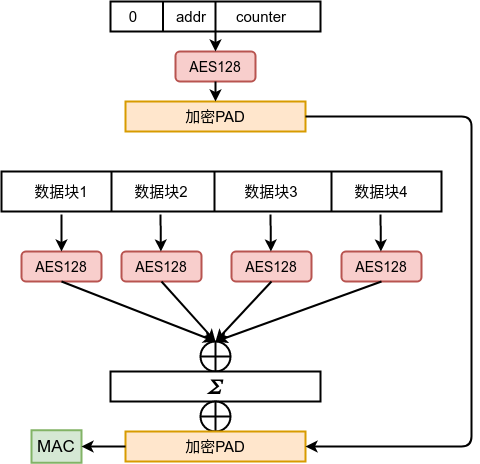
\includegraphics[scale=0.6]{PMAC.png}
  \caption{\textbf{PMAC:}并行计算数据块MAC}
 \label{fig:PMAC.png}
\end{figure}

如图~\ref{fig:PMAC.png}所示,在PMAC中,会将数据块划分成为等长M块,其中的每一块数据的长度都是,e.g., 128 bit,同时PMAC还生成key1, key2用于AES加密计算。对分割好的M块数据分别用AES(key1)做加密,将加密后得到的M块密文块通过异或的方式生成$\Sigma$。
最后用AES(key2,CTR)得到对应的pad(其中CTR为内存的counter和地址),然后对之前得到的$\Sigma$做异或运算,异或后的结果就是PMAC算法最终得到的MAC值。在PMAC的整个过程中,可以对分割好的M块数据同时进行AES加密,相较于CMAC, HMAC这类串行的MAC来说非常的高效,并且AES加密计算本身非常高效,所以PMAC被认为是一种高效的计算MAC函数。

\section{启动阶段}
在内存分布中,我们将内存分成了不可信的内存区域,安全的内存区域,子树节点区域以及MMT元素据据区域。其中只有MMT元数据区域需要在硬件启动的时候就被配置好,剩下的区域能够在之后被动态的分配。在安全启动中,通电之后,在硬件固件中的bootloader会首先被加载运行,首先bootloader会随机生成用于完整性检查的PMAC的两个密钥key1,key2
同时bootloader会根据拥有的内存大小,指定一块区域为MMT元素据区域,并且用PMP将该区域保护起来,只有M mode程序能够访问该区域。之后bootloader会加载monitor的代码。因为monitor的代码需要完整性保护,所以bootloader需要将monitor所在的内存区域设置为安全内存区域,同时为monitor分配对应的子树的节点空间,将初始化的子树根节点哈希和地址填到对应的MMT元数据区域中,更新根数中的哈希值。之后将monitor的代码加载到安全内存中,同时更新对应的子树的哈希值。
bootloader加载完monitor的代码后,计算monitor中的代码的哈希,用于之后的验证。然后将控制权转交给monitor,由monitor进行之后的启动代码。因此在bootloader启动的时候内存中的布局为:由bootloader中配置到的MMT元数据区域,由bootloader分配的monitor的安全内存区域以及对应的子树节点区域。在MMT元数据区域中分配第一个子树用于保护monitor中的内存。
当monitor启动之后,会按照需求,分配剩下的安全内存以及对应的子树,然后把对应的子树的根节点添加到MMT元数据区域中。整个安全启动的可信链为可信的bootloader(硬件的固件中,通常不能够更新或者只能更新厂家提供的bootloader),bootloader配置MMT 元数据区域以及monitor的安全内存,同时验证了monitor的代码的完整性。这两个操作保证了monitor的运行在安全的内存中
并且monitor代码本身的完整性得到保证,然后运行monitor,monitor的安全bootloader保证,所以monitor被认为时安全,由monitor进行之后的可信内存的配置。

\section{分配子树}
不是所有的安全内存都需要在启动的时候配置,这也是MMT的一个特色即动态的分配安全内存。所以monitor在启动之后会负责分配安全内存以及对应的子树的空间,并且将初始化的子树根节点添加到MMT元数据区域中。
为了保证分配子树的安全。monitor对外暴露特定的monitor call的接口。非M mode的程序只能够通过调用给定的接口在可以配置安全的内存。\emph{SBI\_ALLOC\_SECURE\_MEMORY(addr, len)}该接口用于将[addr, addr+len]的内存设置为需要安全内存,如果该内存区域已经为安全内存,那么将忽略之后的步骤
monitor在分配的过程会从自己的内存中或者向kernel中索要一块内存用于存放该安全内存的子树节点。monitor可以按照需将将安全内粗清零或者根据已有的数据计算出当前的子树中各节点的哈希值,然后将子树的
根节点的哈希值以及对应的子树节点的地址填入MMT 元数据区域中。然后monitor通过一条特殊的指令将内存控制器中的secure bitmap中对应的子树设置为1,代表该子树处于已分配的状态。\emph{SBI\_FREE\_SECURE\_MEMORY(addr, len)},首先monitor会通过
内存控制器中的secure bitmap检查当前的内存区域是否时安全内存区域,如果当前内存不是安全内存那么将忽略之后的步骤。monitor会清楚该内存在seucre bitmap的中的标志。如果内存对应的子树在Mount table中,则会将当前该子树的根节点驱逐初Mount table中。同时会清空
MMT 元数据区域中的对应的子树的根节点的哈希值和地址,同时清除子树节点中改的数据,防止信息泄露。通过这两个特殊的SBI call我们可以实现mountable merkle tree中的两个动态原语:添加(add)和移除(remove)。通过这两个动态原语
我们可以实现动态的安全内存分配以及离散的内存保护。不需要再初始化的时候,就将所有的树的节点的内存空间分配好。树的节点所占用的内存空间为保护数据的大小的15-25\%,在云场景下,这部分的内存开销不可以忽略,特别时当需要保护的内存较少,非安全内存的较多的情况,子树节点的
内存未被使用,但是也不能作为正常的非安全内存共程序使用。所以MMT提供了一种更加灵活的内存保护方案,尽量的减少额外的内存开销,提供了较高的可扩展性。

\section{细粒度保护}
之前我们所讨论的对内存的完整性保护的粒度都是以子树的粒度进行,但是子树的大小在不同的实现中并不一致(在本论文中子树的大小未4M),这给上层的操作系统带来内存管理的不便。同时子树的粒度与页粒度相比较大,不利于细粒度的内存管理,所以我们希望能够有一种更加细粒度的完全内存的划分方式。
Mountable merklr tree可以支持更加细粒度的内存保护(最小为缓存行级64B)。为了实现更细粒度的内存保护,需要软硬间结合实现,而不能仅仅靠内存控制器实现。在软件方面monitor可以通过tag memory或者控制页表等方式实现也页粒度的内存隔离,同时赋予CPU两个模式:安全模式与非安全模式。我们认为
在安全模式下,CPU访问的内存都是安全内存,在非安全模式下,CPU访问的内粗都是非安全内存。这样在内存控制器中就不需要关心访问的内存是否安全。但是由于挂载的单位是子树,如果子树的粒度为页大小,会导致子树过多,频繁的发生挂载与卸载的操作。如果不改变子树的大小,那么在一棵子树中,必然同时存在安全内存以及非安全内存。
对于安全内存的访问,我们还是按照上面所说的完整性检查的流程进行。对于子树中的非安全内存,我们将其对应的counter全部设置为一个常量,对该内存的读写都不会去修改对应的counter的数值,而对安全内存的读写中会将非安全内存的counter当作一个常量加载进来,作为PMAC输入参数的一部分,进行完整性计算与验证。
因为非安全内存对应的counter不会发生改变,所以并不影响安全内存的检验。当我们希望将非安全内存转换为安全内存的时候,我们可以将之前设置的常量counter作为初始值,结合非安全内存中的初始数据计算对应的哈希值,然后更新子树的根节点中的哈希值。通过这样的方式能够将非安全内存转换为安全内存,同时并不影响原有的安全内存的检查。

\section{总结}
在本论文中,我们提出了可挂载完整性保护树,哈希森林,子树与根数等概念,并且提出了四个完整性保护树的动态原语:挂载(Mount),卸载(Unmount),添加(add)与移除(remove)。另外通过观察我们发现了内存访问的存在局域性,冷热不平衡的现象,通过设计Mount Table,三层counter等结构来解决内存访问不平衡的问题。
我们在RISCV架构上实现了MMT的原型,它能够实现了对离散内存的完整性保护,支持动态的分配安全内存,同时将支持TB级别的内存完整性保护。可挂载完整性保护树能够兼容已有的完整性保护的数据结构,可以很方便的移植到现有的方案中。同时只需要对内存控制器做一定的修改,对CPU核心的修改较小,能够适应
不同的指令集架构。可挂载完整性保护树的提出能够适应多种新型的应用场景,包括了具有高安全需求的可行执行环境TEE,以及新型的内存存储NVM中。为解决内存完整性保护提供了新的支持




